\documentclass{article}
\usepackage{ctex}
\usepackage{graphicx}
\usepackage{amsmath}
\usepackage{indentfirst}
\usepackage{titlesec}
\usepackage{setspace}
\usepackage{subfigure}
\usepackage{caption}
\usepackage{float}
\usepackage{booktabs}
\usepackage{geometry}
\usepackage{multirow}
\usepackage{hyperref}
\hypersetup{
	colorlinks=true,
	linkcolor=blue,
	filecolor=magenta,      
	urlcolor=cyan,
	pdftitle={Overleaf Example},
	pdfpagemode=FullScreen,
}
\geometry{left=1.2cm,right=1.2cm,top=2cm,bottom=2cm}
\title{\songti \zihao{2}\bfseries 石墨烯态密度计算}
\titleformat*{\section}{\songti\zihao{4}\bfseries}
\titleformat*{\subsection}{\songti\zihao{5}\bfseries}
\renewcommand\thesection{\arabic{section}}
\author{王启骅 PB20020580}
\begin{document}
	\maketitle
\section{自由电子情况}
石墨烯结构为六角晶胞如图\ref{fig:1},边长为a,面积$ S=\frac{3\sqrt{3}}{2}a^2 $,一个原胞中存在两种原子,其中红色和绿色各一种。
	\begin{figure}[!h]
	
	\centering
	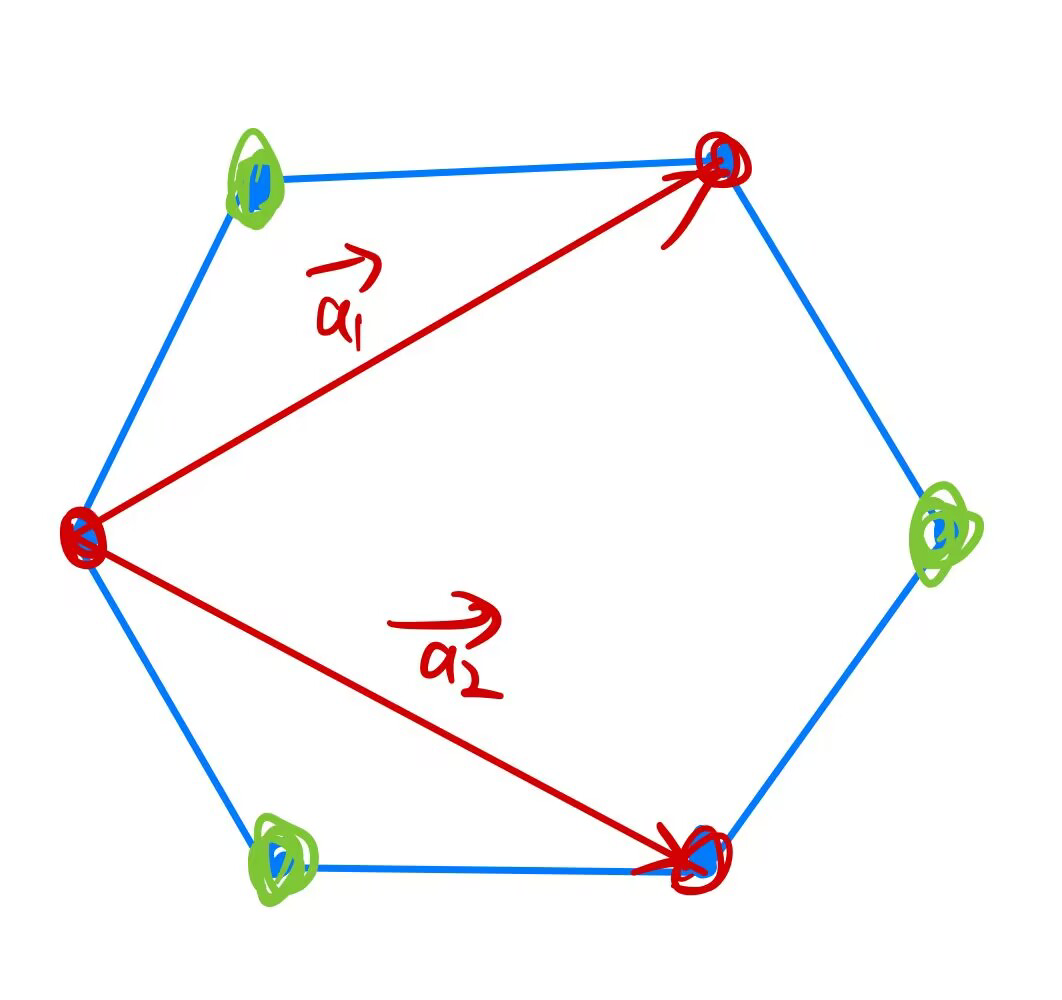
\includegraphics[scale=0.25]{晶胞}
	\captionsetup{font={small},labelfont=bf}
	\caption{\heiti\zihao{-5}石墨烯晶胞}
	\label{fig:1}
\end{figure}
可以得到平移不变的矢量
\begin{equation}
	\begin{cases}
		\vec{a_1}=\frac{3}{2}a\hat{x}+\frac{\sqrt{3}}{2}a\hat{y}\\
		\vec{a_2}=\frac{3}{2}a\hat{x}-\frac{\sqrt{3}}{2}a\hat{y}
	\end{cases}
\end{equation}
根据周期性边界条件
\begin{equation}
		\psi(x,y)=\psi(x+\frac{3}{2}a,y\pm\frac{\sqrt{3}}{2}a)
\end{equation}
得到波矢满足条件
\begin{equation}
	\exp(i\vec{k}\cdot\vec{a_1})=\exp(i\vec{k}\cdot\vec{a_2})=1
\end{equation}
得到
\begin{equation}
	\begin{cases}
		k_x=\frac{2\pi}{3a}(n_1+n_2)\\
		k_y=\frac{2\pi}{\sqrt{3}a}(n_1-n_2)
	\end{cases}
\end{equation}
则波矢k空间中可以取得的点为
	\begin{figure}[!h]
	
	\centering
	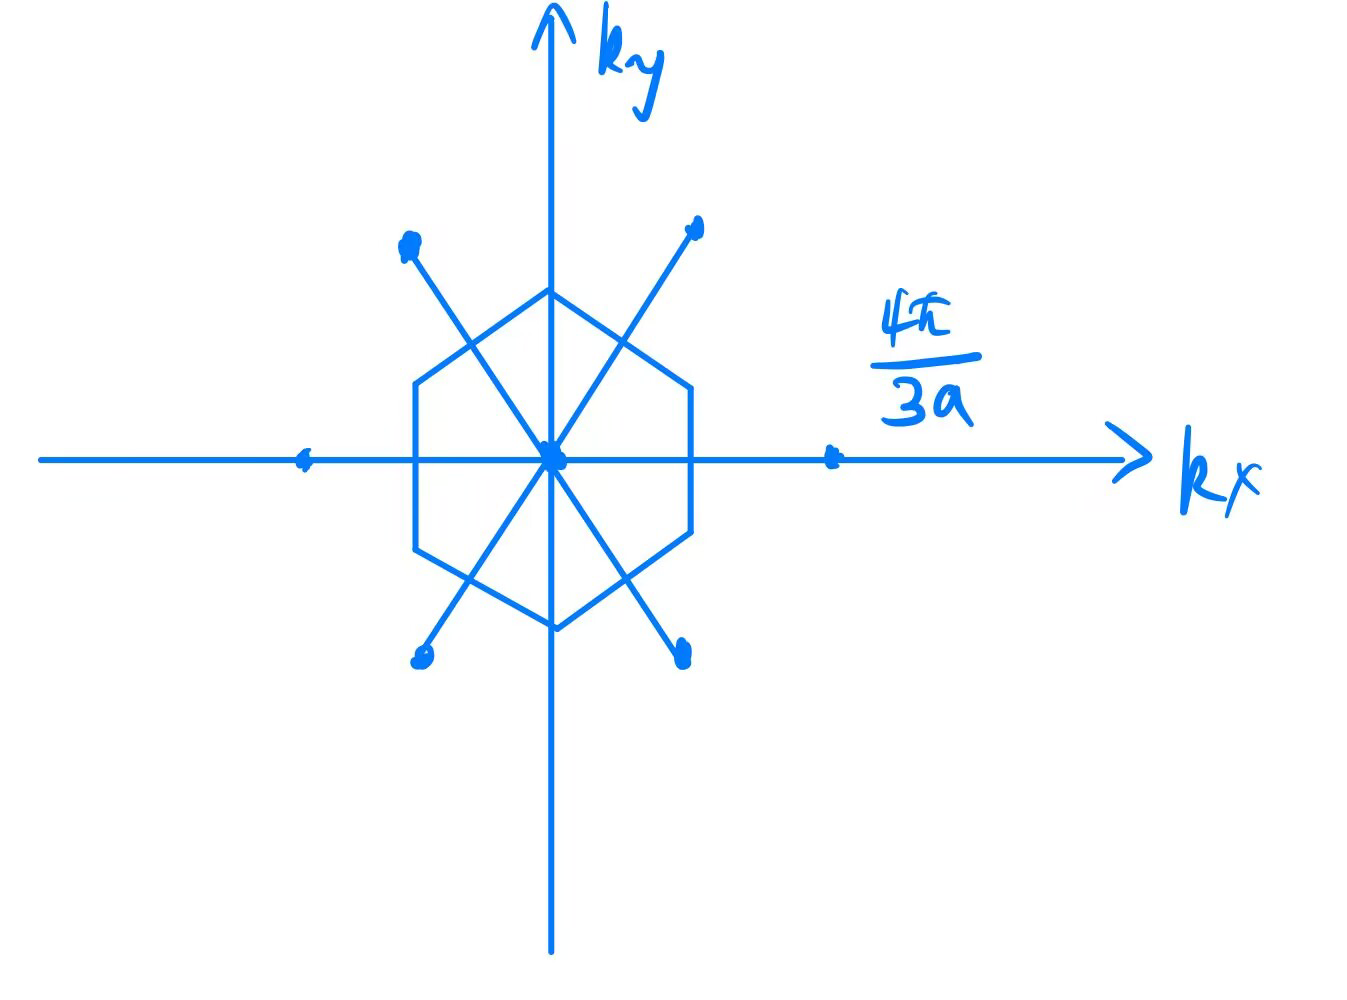
\includegraphics[scale=0.2]{k空间}
	\captionsetup{font={small},labelfont=bf}
	\caption{\heiti\zihao{-5}k空间电子态分布}
	\label{fig:2}
\end{figure}
一个态所占的面积为$ \Delta\vec{k}=\frac{8\pi^2}{3\sqrt{3}a^2}=\frac{4\pi^2}{S} $,由k空间中电子态均匀分布,
\begin{equation}
	\rho(k)=\frac{S}{4\pi^2}
\end{equation}
在半径为k的圆中,能态总数
\begin{equation}
	Z(E)=2\rho(k)\pi k^2=S\frac{mE}{\pi\hbar^2}
\end{equation}
可得态密度
\begin{equation}
	N(E)=\dfrac{d\frac{Z}{S}}{dE}=\frac{m}{\pi\hbar^2}
\end{equation}


可见该态密度为常数,与E无关。

\section{紧束缚近似}
由于自由电子情况下态密度为常数,接下来进一步考虑紧束缚近似下的态密度。对于石墨烯,一个原胞中含有两个原子。取晶体原胞所组成的点阵由图\ref{fig:3}
	\begin{figure}[!h]
	
	\centering
	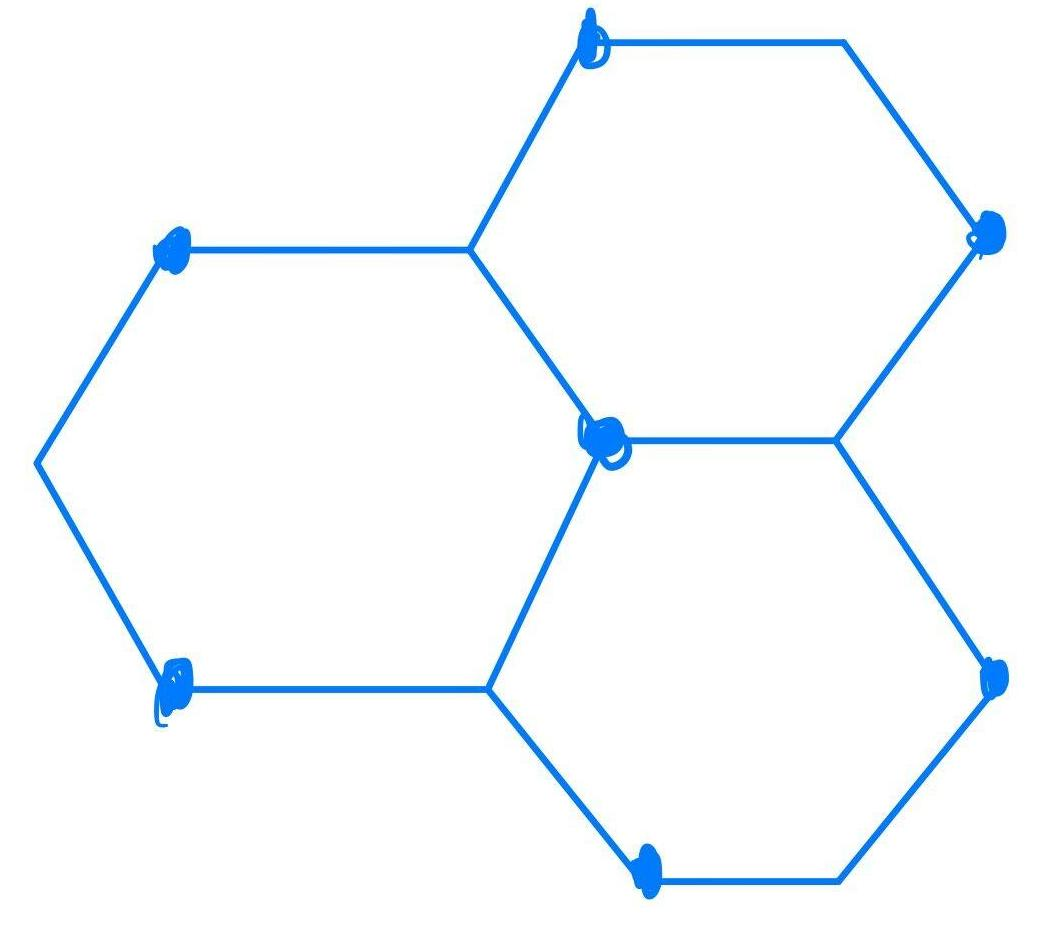
\includegraphics[scale=0.2]{原胞点阵}
	\captionsetup{font={small},labelfont=bf}
	\caption{\heiti\zihao{-5}石墨烯原胞点阵}
	\label{fig:3}
\end{figure}

考虑最近邻原胞的作用,
\begin{equation}
	\begin{aligned}
	E&=E_0-J_1\big(\exp(-\i(k_x\frac{3}{2}a+k_y\frac{\sqrt{3}}{3}a))+\exp(-\i(k_x\frac{3}{2}a-k_y\frac{\sqrt{3}}{3}a))+\exp(-\i k_y\sqrt{3}a)+\exp(\i k_y\sqrt{3}a)\\
	&+\exp(-\i(-k_x\frac{3}{2}a+k_y\frac{\sqrt{3}}{3}a))+\exp(-\i(-k_x\frac{3}{2}a-k_y\frac{\sqrt{3}}{3}a))\big)\\
	&=E_0-2J_1\big(2\cos(\frac{3}{2}ak_x)\cos(\frac{\sqrt{3}}{2}ak_y)+\cos(\sqrt{3}ak_y)\big)
	\end{aligned}
\end{equation}
\begin{equation}
	\nabla_kE=2J_1\big(3a\sin(\frac{3}{2}ak_x)\cos(\frac{\sqrt{3}}{2}ak_y)\hat{k_x}+\sqrt{3}a\cos(\frac{3}{2}ak_x)\sin(\frac{\sqrt{3}}{2}ak_y)\hat{k_y}+\sqrt{3}a\sin(\sqrt{3}ak_y)\hat{k_y}\big)
\end{equation}
则可得到能态密度
\begin{equation}
	\begin{aligned}
		N(E)&=\frac{2}{4\pi^2}\int_{E}\frac{dl}{|\nabla_kE|}\\
		&=\frac{1}{4\pi^2aJ_1}\int_{E}\frac{dl}{\sqrt{9\sin^2(\frac{3}{2}ak_x)\cos^2(\frac{\sqrt{3}}{2}ak_y)+3(\cos(\frac{3}{2}ak_x)\sin(\frac{\sqrt{3}}{2}ak_y)+\sin(\sqrt{3}ak_y))^2}}
	\end{aligned}
\end{equation}
该积分沿等能线E进行,即可得到在该能量下的能态密度。
\end{document}